\documentclass[10pt]{beamer}

%STANDARD PREAMBLE
%https://tex.stackexchange.com/questions/68821/is-it-possible-to-create-a-latex-preamble-header
\usepackage{/Users/mwojno01/Repos/latex_preamble/beamer_preamble}

%%%
% SPECIFIC TO THIS DOCUMENT
%%%
% FASTER LIMITS, INTEGRALS AND SUMS
\newcommand{\dlim}{\ds\lim}
\newcommand{\dint}{\ds\int}
\newcommand{\dsum}{\ds\sum}
\newcommand{\dmu}{\wrt{\mu}}

% SUBFIGURES
\usepackage{subcaption}

%
%% ALLOW FOR ITEMIZE ENVIRONMENTS WITH NO PRECEDING
% SPACING, IF DESIRED
% Reference: https://tex.stackexchange.com/questions/86054/how-to-remove-the-whitespace-before-itemize-enumerate
%\usepackage{enumitem}% http://ctan.org/pkg/enumitem 
\usepackage{paralist}

\title{Counting Measure and Stationary Time Series}

\begin{document}

\maketitle

\begin{frame}[standout]
 Measure theory is convenient in unifying various kinds of random variables.	
 \vfill
 \small{In this lightning chat, I give a real example that came up when investigating time series.}
\end{frame}


\begin{frame}{Table of contents}
  \setbeamertemplate{section in toc}[sections numbered]
  \tableofcontents[hideallsubsections]
\end{frame}

\section{Series as integrals against counting measure}

\begin{frame}{Measure spaces}
A measure space $(\Omega, \F, \mu)$ consists of

\begin{enumerate}
\item Some set $\Omega$.
\item A sigma-field $\F$, which specifies \textit{measurable} subsets of $\Omega$.
\item A measure $\mu$.	
\end{enumerate}

\vfill 
 
Example measures
 \begin{itemize}
 \item 
 \textit{Lebesgue measure.} This gives the length of intervals  
\[ \mu(a,b] = b-a \quad \forall \, a,b \in \R : b>a \]
but can be used to measure other kinds of sets.
\item \textit{Counting measure}. This gives the number of points a set.
 \end{itemize}

\end{frame}

\begin{frame}{Integrals of simple functions}

\vfill 
\begin{definition}
Let $(\Omega, \F, \mu)$ be a measure space. Then $s$ is a \textbf{simple function} if we can write 
\[s = \sum_{i=1}^n c_i \indicate{A_i} \] 
where $\indicate{}$ is the indicator function and the $A_i$ are disjoint sets in $\F$. 
\end{definition}

\vfill 
\begin{block}{Definition}
Let $s = \sum_{i=1}^n c_i \indicate{A_i}$ be a simple function. Then the \textbf{integral of a simple function} is defined as
%
\begin{align*}
\ds\int_\Omega s \wrt{\mu} := \ds\sum_{i=1}^n c_i \; \mu(A_i).
\labelit \label{eqn:integral_of_simple_function}	
\end{align*}
\end{block}	
\end{frame}

\begin{frame}{Examples of integrals of simple functions}

\begin{figure}[H]
\centering
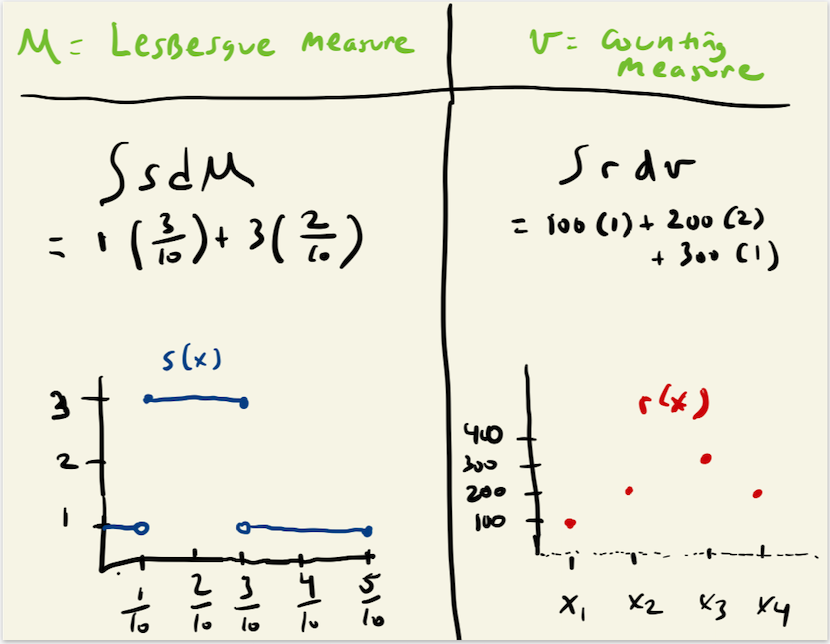
\includegraphics[width=.9\textwidth]{images/examples_of_integrals_of_simple_functions.png}	
\end{figure}
	
\end{frame}

\begin{frame}{Series as integrals against counting measure} 
Let $\Omega = \set{1,2,3, ...}$, $\F=2^\Omega$ (i.e. all subsets of $\Omega$), and $\mu$ be the counting measure. 

\vfill 

A real-valued function $f$ on $\Omega$ can be written as a sequence of real numbers; we write $f=\set{a_n}, n=1,2, \hdots$.  

\vfill 

It can be shown that an integral on this space is really a series:
%
\begin{align*}
\int_\Omega f \wrt{\mu} = \sum_{n=1}^\infty a_n	
%\label{eqn:sums_as_integrals}
\end{align*}	
\end{frame}

\begin{frame}{Why do we care?}
We can uniformly apply everything we know about integration regardless of whether our space is Euclidean, discrete, or something more exotic.

In the next section, we'll exploit this fact by applying:

\vfill 
\begin{block}{Triangle inequality for integrals}
If $\int_\Omega h \dmu$ exists, then $|\int_\Omega h \dmu| \leq \int_\Omega |h| \dmu$.	
\end{block}

\vfill 

\begin{block}{Tonelli's theorem}
 Suppose that $(X,\F,\mu)$ and $(Y, \G, \nu)$ are $\sigma$-finite measure spaces.   If $f$ is a \alert{non-negative} measurable function on $X \times Y$ then
%
\begin{align*}
\int f \wrt{(\mu \times \nu)} = \int \int f(x,y) \wrt{\nu(y)}   \wrt{\mu(x)}  = \int \int f(x,y) \wrt{\mu(x)}  \wrt{\nu(y)}   
%\label{eqn:classical_fubini_tonelli_equation}
\end{align*}
\end{block}
\end{frame}

\section{Stationary time series}

\begin{frame}{Stationary time series}

Loosely speaking, a time series $\set{X_t, t=0, \pm 1, \hdots }$ is said to be \alert{stationary} if it has statistical properties similar to those of the ``time-shifted" series $\set{X_{t+h}, t=0, \pm 1, \hdots}$ for each integer $h$.
\vfill 

\begin{definition}
A time series $\set{X_t}$ is said to be \textbf{covariance stationary}	if it has finite variance and
%
\begin{align*}
\E[X_t] &=c \qquad \forall t \\
\Cov[X_t, X_{t+h}] &= \gamma(h) \qquad \forall t,h
\end{align*}

\end{definition}
\end{frame}

\begin{frame}{Example of stationary time series}
	
\begin{figure}[t!]
    \centering
    \begin{subfigure}[t]{0.48\textwidth}
        \centering
     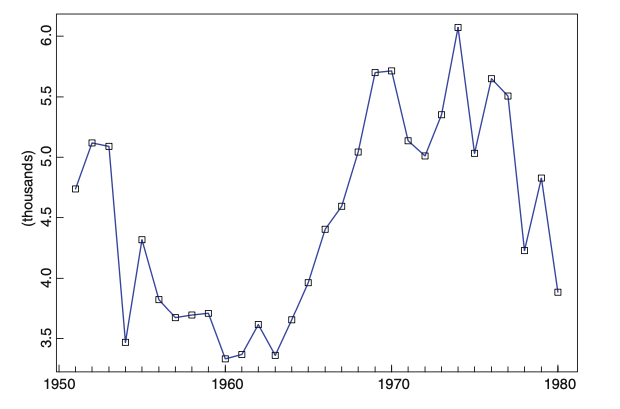
\includegraphics[width=.95\textwidth]{images/strikes_in_USA.png}
        \caption{Strikes in the U.S.A, 1951-1980}
    \end{subfigure}%
    ~ 
    \begin{subfigure}[t]{0.48\textwidth}
        \centering
    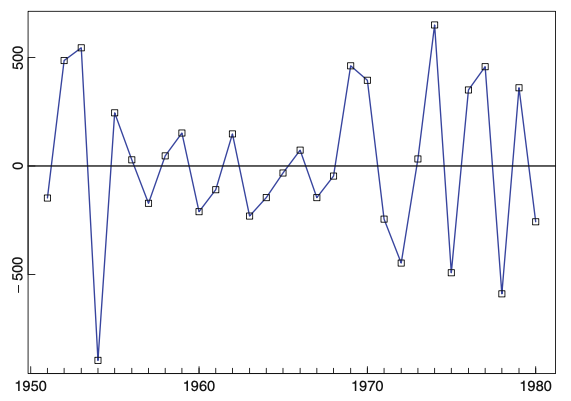
\includegraphics[width=.95\textwidth]{images/strikes_in_USA_after_detrending.png}
        \caption{Strikes in the U.S.A., after detrending}
    \end{subfigure}
    \caption{The time series on the right can be accurately modeled as a stationary time series. Image credits: Brockwell, Peter J., and Richard A. Davis (2016) \textit{Introduction to time series and forecasting.}}
\end{figure}
\end{frame}


\begin{frame}{Linear processes}

A linear process is linearly filtered white noise. 

\vfill 
\begin{definition} 
A process $\{ W_t\}$ is called \textbf{white noise}, denoted $\{W_t\} \sim \text{WN}(0, \sigma^2_W)$, if it is a sequence of uncorrelated random variables with mean 0 and finite variance $\sigma^2$. 
\label{def:white_noise}
\end{definition}

\vfill 

\begin{definition}  \label{def:linear_process_representation}
A time series $X_t$ is said to be a \textbf{linear process} if it has the representation 
%
\begin{align}
X_t = \ds\sum_{j=-\infty}^\infty \psi_j W_{t-j}
\label{eqn:linear_process_representation}
\end{align}
%
for all $t$, where $W_t \sim WN(0, \sigma_W^2)$, and $\{ \psi_j\}$ is a sequence of constants which is absolutely summable ($\sum_{j=0}^\infty  |\psi_j| < \infty$).
\end{definition}
\end{frame}

\begin{frame}{Why do we care?}

\alert{Every} covariance stationary process is either a linear process or can be transformed to one by subtracting a deterministic component.  

This important result is known as Wold's decomposition.
	
\end{frame}

\begin{frame}{Application of general integration theory}  

\begin{block}{Linear processes almost surely converge}
We show that the infinite sum in  \eqref{eqn:linear_process_representation} converges almost surely:
%
\begin{align*}
 \E|X_t| &= \E \bigg|\ds\sum_{j=-\infty}^{j=\infty} \psi_j \, W_{t-j} \bigg| \\
 & \leq \E \ds\sum_{j=-\infty}^{j=\infty} |\psi_j \, W_{t-j}|  && \text{by $\triangle$ inequality} \\
 &= \ds\sum_{j=-\infty}^{j=\infty} |\psi_j| \, \E |W_{t-j}| && \text{by Tonelli} \\
 &\leq \bigg( \ds\sum_{j=-\infty}^{j=\infty} |\psi_j|  \bigg) \sigma_W \\
 &< \infty. 
 \end{align*}
%
Thus, the series defining $X_t$ is almost surely finite. %So $X_t$ almost surely converges absolutely. %So by definition, $X_t$ is almost surely absolutely convergent.

%\footnote{The set of outcomes where $X_t$ is infinite must have probability 0, or else the expectation could not be finite.}
\end{block}	
\end{frame}


\end{document}